\section{Dwi Septiani Tsaniyah (1174003)}
\subsection{Teori}
\subsubsection{Soal No. 1}
\hfill \break
Apa itu fungsi library matplotlib?

\hfill \break
Fungsi dari matplotlib adalah untuk menggambar atau membuat suatu grafik yang hasilnya akan muncul gambar dengan hasil 2D

\subsubsection{Soal No. 2}
\hfill \break
Jelaskan langkah-langkah membuat sumbu X dan Y di matplotlib!

\begin{enumerate}
	\item untuk mempermudah pembuatan nya maka kita buatkan list agar lebih mudah lagi dalam penyimpanan di setiap sumbunya.
contoh nya sebagai berikut : 
\lstinputlisting[firstline=9, lastline=10]{src/6/1174003/T1174003.py}
	
\end{enumerate}
 
\subsubsection{Soal No. 3}
\hfill \break
Jelaskan bagaimana perbedaan fungsi dan cara pakai untuk berbagai jenis(bar, histogram ,scatter ,line, dll) jenis plot di matplotlib!

\begin{enumerate}
	\item \textbf{Bar Graph}
	
	perbedaannya adalah dalam bentuk grafiknya. bentuk grafik yang akan dihasilkan yaitu menurut perintah yang dibuat dalam programnnya
	
	\textbf{Kode Program}
	
    \item line
    Perintah yang digunakan untuk membuat grafik line sebagai berikut.
    \lstinputlisting[firstline=13, lastline=15]{src/6/1174003/T1174003.py}
    \item bar
    Dalam Penggunaan plot bar koordinat x nya itu yang awal, dan untuk Y nya adalah yang kedua
    \lstinputlisting[firstline=16, lastline=25]{src/6/1174003/T1174003.py}
    \item histogram
    Dalam penggunaan plot histogram titik x nya bisa tidak sama dengan titik Y.
    untuk penggunaannya bisa sebagai berikut.
    \lstinputlisting[firstline=27, lastline=34]{src/6/1174003/T1174003.py}
    \item scatter
    Untuk penggunaa plot scatter atau bisa juga d bilang diagram titik.
    Contoh dari penggunaannya bisa dilihat sebagai berikut.
    \lstinputlisting[firstline=36, lastline=49]{src/6/1174003/T1174003.py}
    \item Stack plot
    Untuk penggunaan stack plot ini seperti diagram line, tapi ada fill colornya,jadi antar line itu bisa berdekatan.
    Berikut Contoh penggunaannya
    \lstinputlisting[firstline=82, lastline=92]{src/6/1174003/T1174003.py}
	
\end{enumerate}

\subsubsection{Soal No. 4}
\hfill \break
Jelaskan bagaimana cara menggunakan legend dan label serta kaitannya dengan fungsi tersebut!

\hfill \break
Untuk menggunakan sebuah lagend bisa menggunakan program seperti dibawah ini :
\lstinputlisting[firstline=20, lastline=22]{src/6/1174003/T1174003.py}
Penggunaan legend sendiri adalah untuk mempermudah kita dalam membaca suatu grafik yang telah dibuat.
dan untuk membedakan X dan Y menggunakan label

\subsubsection{Soal No. 5}
\hfill \break
Jelaskan apa fungsi dari subplot di matplotlib, dan bagaimana cara kerja dari fungsi subplot, sertakan ilustrasi dan gambar sendiri dan apa parameternya jika ingin menggambar plot dengan 9 subplot di dalamnya!

\hfill \break
fungsi dari sebuah subplot yaitu bisa menggambarkan lebih dari 1 grafik dengan 1 program saja.
untuk cara kerja nya dapat dilihat dengan contoh dibawah ini :
\lstinputlisting[firstline=94, lastline=104]{src/6/1174003/T1174003.py}

\subsubsection{Soal No. 6}
\hfill \break
Sebutkan semua parameter color yang bisa digunakan (contoh:  m,c,r,k,...  dkk)!

\begin{itemize}
    \item Tipe Warna RGB
    Untuk keterangannya sebagai berikut
    R untuk warna Red atau Merah
    G untuk warna Green atau Hijau
    B untuk warna Blue atau Biru
    \item Tipe warna CMYK
    Untuk keterangannya sebagai berikut
    C untuk warna Cyan atau Biru Muda
    M untuk warna Mangenta atau Merah Tua
    Y untuk warna Yellow Atau Kuning
    K untuk warna blacK atau Hitam
\end{itemize}

\subsubsection{Soal No. 7}
\hfill \break
Jelaskan bagaimana cara kerja dari fungsi hist, sertakan ilustrasi dan gambar sendiri!

\hfill \break
untuk fungsi histogram sendiri yaitu kedua koordinat nya tidak boleh sama .
Ini merupakan contoh dari penggunaan histogram
\lstinputlisting[firstline=28, lastline=35]{src/6/1174003/T1174003.py}
dan ini merupakan grafik histogram tersebut.
\begin{figure}[H]	
    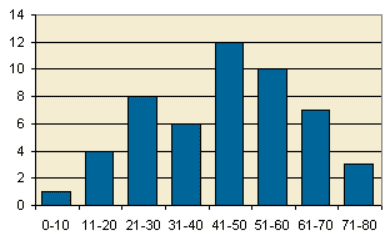
\includegraphics[width=5cm]{figures/6/1174003/histogram.png}
    \centering
    \caption{Diagram Histogram}
\end{figure}

\subsubsection{Soal No. 8}
\hfill \break
 Jelaskan lebih mendalam tentang parameter dari fungsi pie diantaranya labels, colors, startangle, shadow, explode, autopct!
 
\hfill \break
Berikut penjelasan tentang parameter yang ada dalam pie chart
\begin{itemize}
    \item label
	mempermudah untuk membaca diagram pie
    \item color
    untuk membedakan suatu data
    \item startangle
    Digunakan untuk sudut yang digunakan untuk memulai diagram pie tersebut
    \item shadow
    membuat bayangan disetiap pie yang menonjol
    \item explode
    digunakan untuk mengeluarkan suatu data agar terlihat meninjol
    \item autopct
    Digunakan sesuai dengan berapa angka dibelakang koma
\end{itemize}

\subsection{Praktek}
\subsubsection{soal 1}
 Buatlah librari fungsi (file terpisah/library dengan nama NPM bar.py) untuk plot dengan jumlah subplot adalah NPM mod 3 + 2
\lstinputlisting[firstline=8, lastline=28]{src/6/1174003/c1174003_bar.py}
untuk memunculkan hasilnya kita dapat memanggil menggunakan :
\lstinputlisting[firstline=8, lastline=8]{src/6/1174003/main_dwis.py}
\lstinputlisting[firstline=13, lastline=13]{src/6/1174003/main_dwis.py}
dan akan menghasilkan grafik seperti gambar berikut:
\begin{figure}[H]
\centering
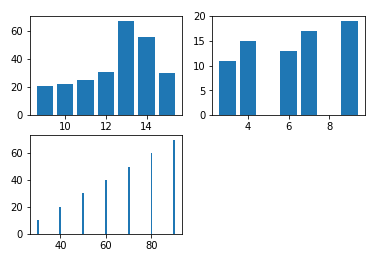
\includegraphics[width=7cm]{figures/6/1174003/p1.png}
\caption{Grafik Batang}
\label{dwisep}
\end{figure}

\subsubsection{soal 2}
Buatlah librari fungsi (file terpisah/library dengan nama NPM scatter.py) untuk plot dengan jumlah subplot NPM mod 3 + 2
\lstinputlisting[firstline=8, lastline=28]{src/6/1174003/d1174003_scat.py}
untuk memunculkan hasilnya kita dapat memanggil menggunakan :
\lstinputlisting[firstline=9, lastline=9]{src/6/1174003/main_dwis.py}
\lstinputlisting[firstline=14, lastline=14]{src/6/1174003/main_dwis.py}
dan akan menghasilkan grafik seperti gambar berikut:
\begin{figure}[H]
\centering
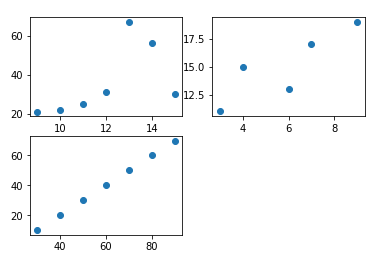
\includegraphics[width=7cm]{figures/6/1174003/p2.png}
\caption{Grafik Scat}
\label{dwisep}
\end{figure}


\subsubsection{soal 3}
Buatlah librari fungsi (file terpisah/library dengan nama NPM pie.py) untuk plot dengan jumlah subplot NPM mod 3 + 2
\lstinputlisting[firstline=8, lastline=50]{src/6/1174003/c1174003_pie.py}
untuk memunculkan hasilnya kita dapat memanggil menggunakan :
\lstinputlisting[firstline=10, lastline=10]{src/6/1174003/main_dwis.py}
\lstinputlisting[firstline=15, lastline=15]{src/6/1174003/main_dwis.py}
dan akan menghasilkan grafik seperti gambar berikut:
\begin{figure}[H]
\centering
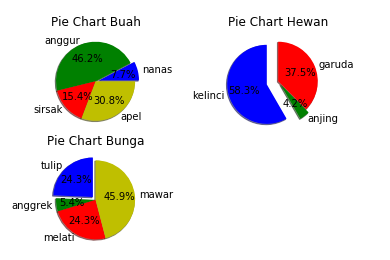
\includegraphics[width=7cm]{figures/6/1174003/p3.png}
\caption{Grafik Pie}
\label{dwisep}
\end{figure}


\subsubsection{soal 4}
Buatlah librari fungsi (file terpisah/library dengan nama NPM plot.py) untuk plot dengan jumlah subplot NPM mod 3 + 2
\lstinputlisting[firstline=8, lastline=28]{src/6/1174003/d1174003_plot.py}
untuk memunculkan hasilnya kita dapat memanggil menggunakan :
\lstinputlisting[firstline=11, lastline=11]{src/6/1174003/main_dwis.py}
\lstinputlisting[firstline=16, lastline=16]{src/6/1174003/main_dwis.py}
dan akan menghasilkan grafik seperti gambar berikut:
\begin{figure}[H]
\centering
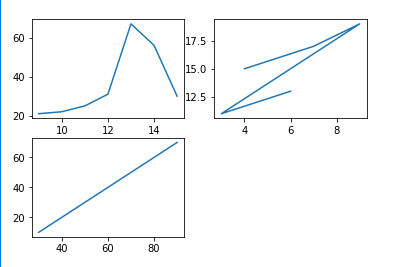
\includegraphics[width=7cm]{figures/6/1174003/p4.png}
\caption{Grafik Plot}
\label{dwisep}
\end{figure}

\subsection{Penanganan Eror}
Apabila terjadi suatu ke-eror-an maka dapat ditangani dengan cara sebagai berikut :
\lstinputlisting[firstline=8, lastline=14]{src/6/1174003/eror.py}